% !TeX root = vortrag
\documentclass[aspectratio=1610]{beamer}
\usetheme{default}
\usecolortheme{dove}
\usepackage[utf8]{inputenc}
\renewcommand{\Re}{\operatorname{\mathbb{R}e}}
\renewcommand{\Im}{\operatorname{\mathbb{I}m}}

%Information to be included in the title page:
\title{Aufbau und Justage eines Leckstrahlmikroskopes zum Nachweis des plasmonischen Spin-Hall-Effektes}
\subtitle{Bachelorarbeit}
\author{Hanno Christiansen}
\institute{Christian-Albrechts-Universität zu Kiel}
\date{2021}

\addtobeamertemplate{navigation symbols}{}{%
	\usebeamerfont{footline}%
	\usebeamercolor[fg]{footline}%
	\hspace{1em}%
	\insertframenumber/\inserttotalframenumber
}



\begin{document}
	
	\frame{\titlepage}
	
	\begin{frame}
		\frametitle{Gliederung}
		\tableofcontents
	\end{frame}

	\section{Theorie}
		\subsection{Surface Plasmon Polariton (SPP)}	
		\begin{frame}
			\frametitle{Surface Plasmon Polariton (SPP)}	
				\begin{center}
					\includegraphics[width=0.7\textwidth]{figures/E_Feld_SPP.png}	
				\end{center}			
		\end{frame}
	
		\begin{frame}
			\frametitle{Orientierung der Felder}
				\begin{subequations}
				\begin{equation}
					\vec{E}_n = \begin{pmatrix} 1 \\ 0 \\ \pm k_{\mathrm{spp}}/k_{z,n} \end{pmatrix} E_0 \exp\left(i(k_{\mathrm{spp}}x + k_{z, n}|z|-\omega t)\right)	
				\end{equation}
				\begin{equation}
					\vec{H}_n = \begin{pmatrix} 0 \\ 1 \\ 0 \end{pmatrix} H_0 \exp\left(i(k_{\mathrm{spp}}x + k_{z, n}|z|-\omega t)\right)
				\end{equation}
			\end{subequations}
		\end{frame}
	
		\begin{frame}
			\frametitle{Dispersion SPP}
			\begin{equation}
				\boxed{k_{\mathrm{spp}}\left(\omega\right) = \dfrac{\omega}{c} \sqrt{\dfrac{\epsilon_D\epsilon_M(\omega)}{\epsilon_D + 	\epsilon_M(\omega)}}  = k_0(\omega) n_{\mathrm{eff}}(\omega)}
			\end{equation}	
		\end{frame}	
		
		\begin{frame}
		\frametitle{Dispersion SPP}
			\begin{center}
				\includegraphics[width=0.7\textwidth]{figures/dispersion.png}
			\end{center}
		\end{frame}
	
		\begin{frame}
		\frametitle{Kretschmann-Konfiguration}
			\begin{center}
				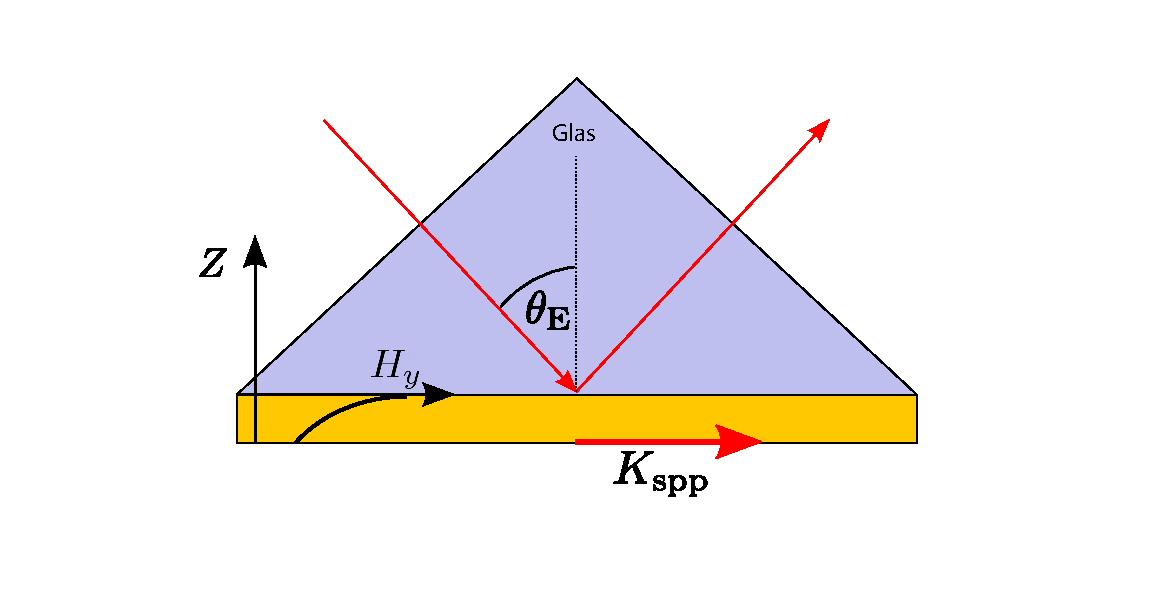
\includegraphics[width=0.7\textwidth]{figures/Kretschmann.pdf}
			\end{center}
		\begin{align}
			\sin(\theta_E) &= \dfrac{\Re\{k_{\mathrm{spp}}\}}{k_{D_1}}\\
			\Rightarrow \Re\{k_{\mathrm{SPP}}\} &= \sin(\theta_E) k_0 \sqrt{\epsilon_{D_1}}
		\end{align}
		\end{frame}
	
		\begin{frame}
			\frametitle{Leckstrahlung}
				\begin{center}
					\includegraphics[width=0.7\textwidth]{figures/leckstrahlung.pdf}
				\end{center}
			\begin{equation}
				\boxed{\Re\{k_{\mathrm{spp}}\}=\sin(\theta_\mathrm{L}) k_0 \sqrt{\epsilon_{D_1}}}
			\end{equation}
		\end{frame}	
		
	
	

		\subsection{Plasmonischer Spin-Hall-Effekt (PSHE)}
			\begin{frame}
				\frametitle{Spin von elektromagnetischer Strahlung}
				\begin{figure}[h]
					\centering
					\includegraphics[width=0.7\linewidth]{figures/spin/prop_spin}
				\end{figure}
				\begin{figure}[h]
					\centering
					\includegraphics[width=0.7\linewidth]{figures/spin/ev_spin}
				\end{figure}				
			\end{frame}
		
		\begin{frame}
			\frametitle{Drehimpulserhaltung beim PSHE}
				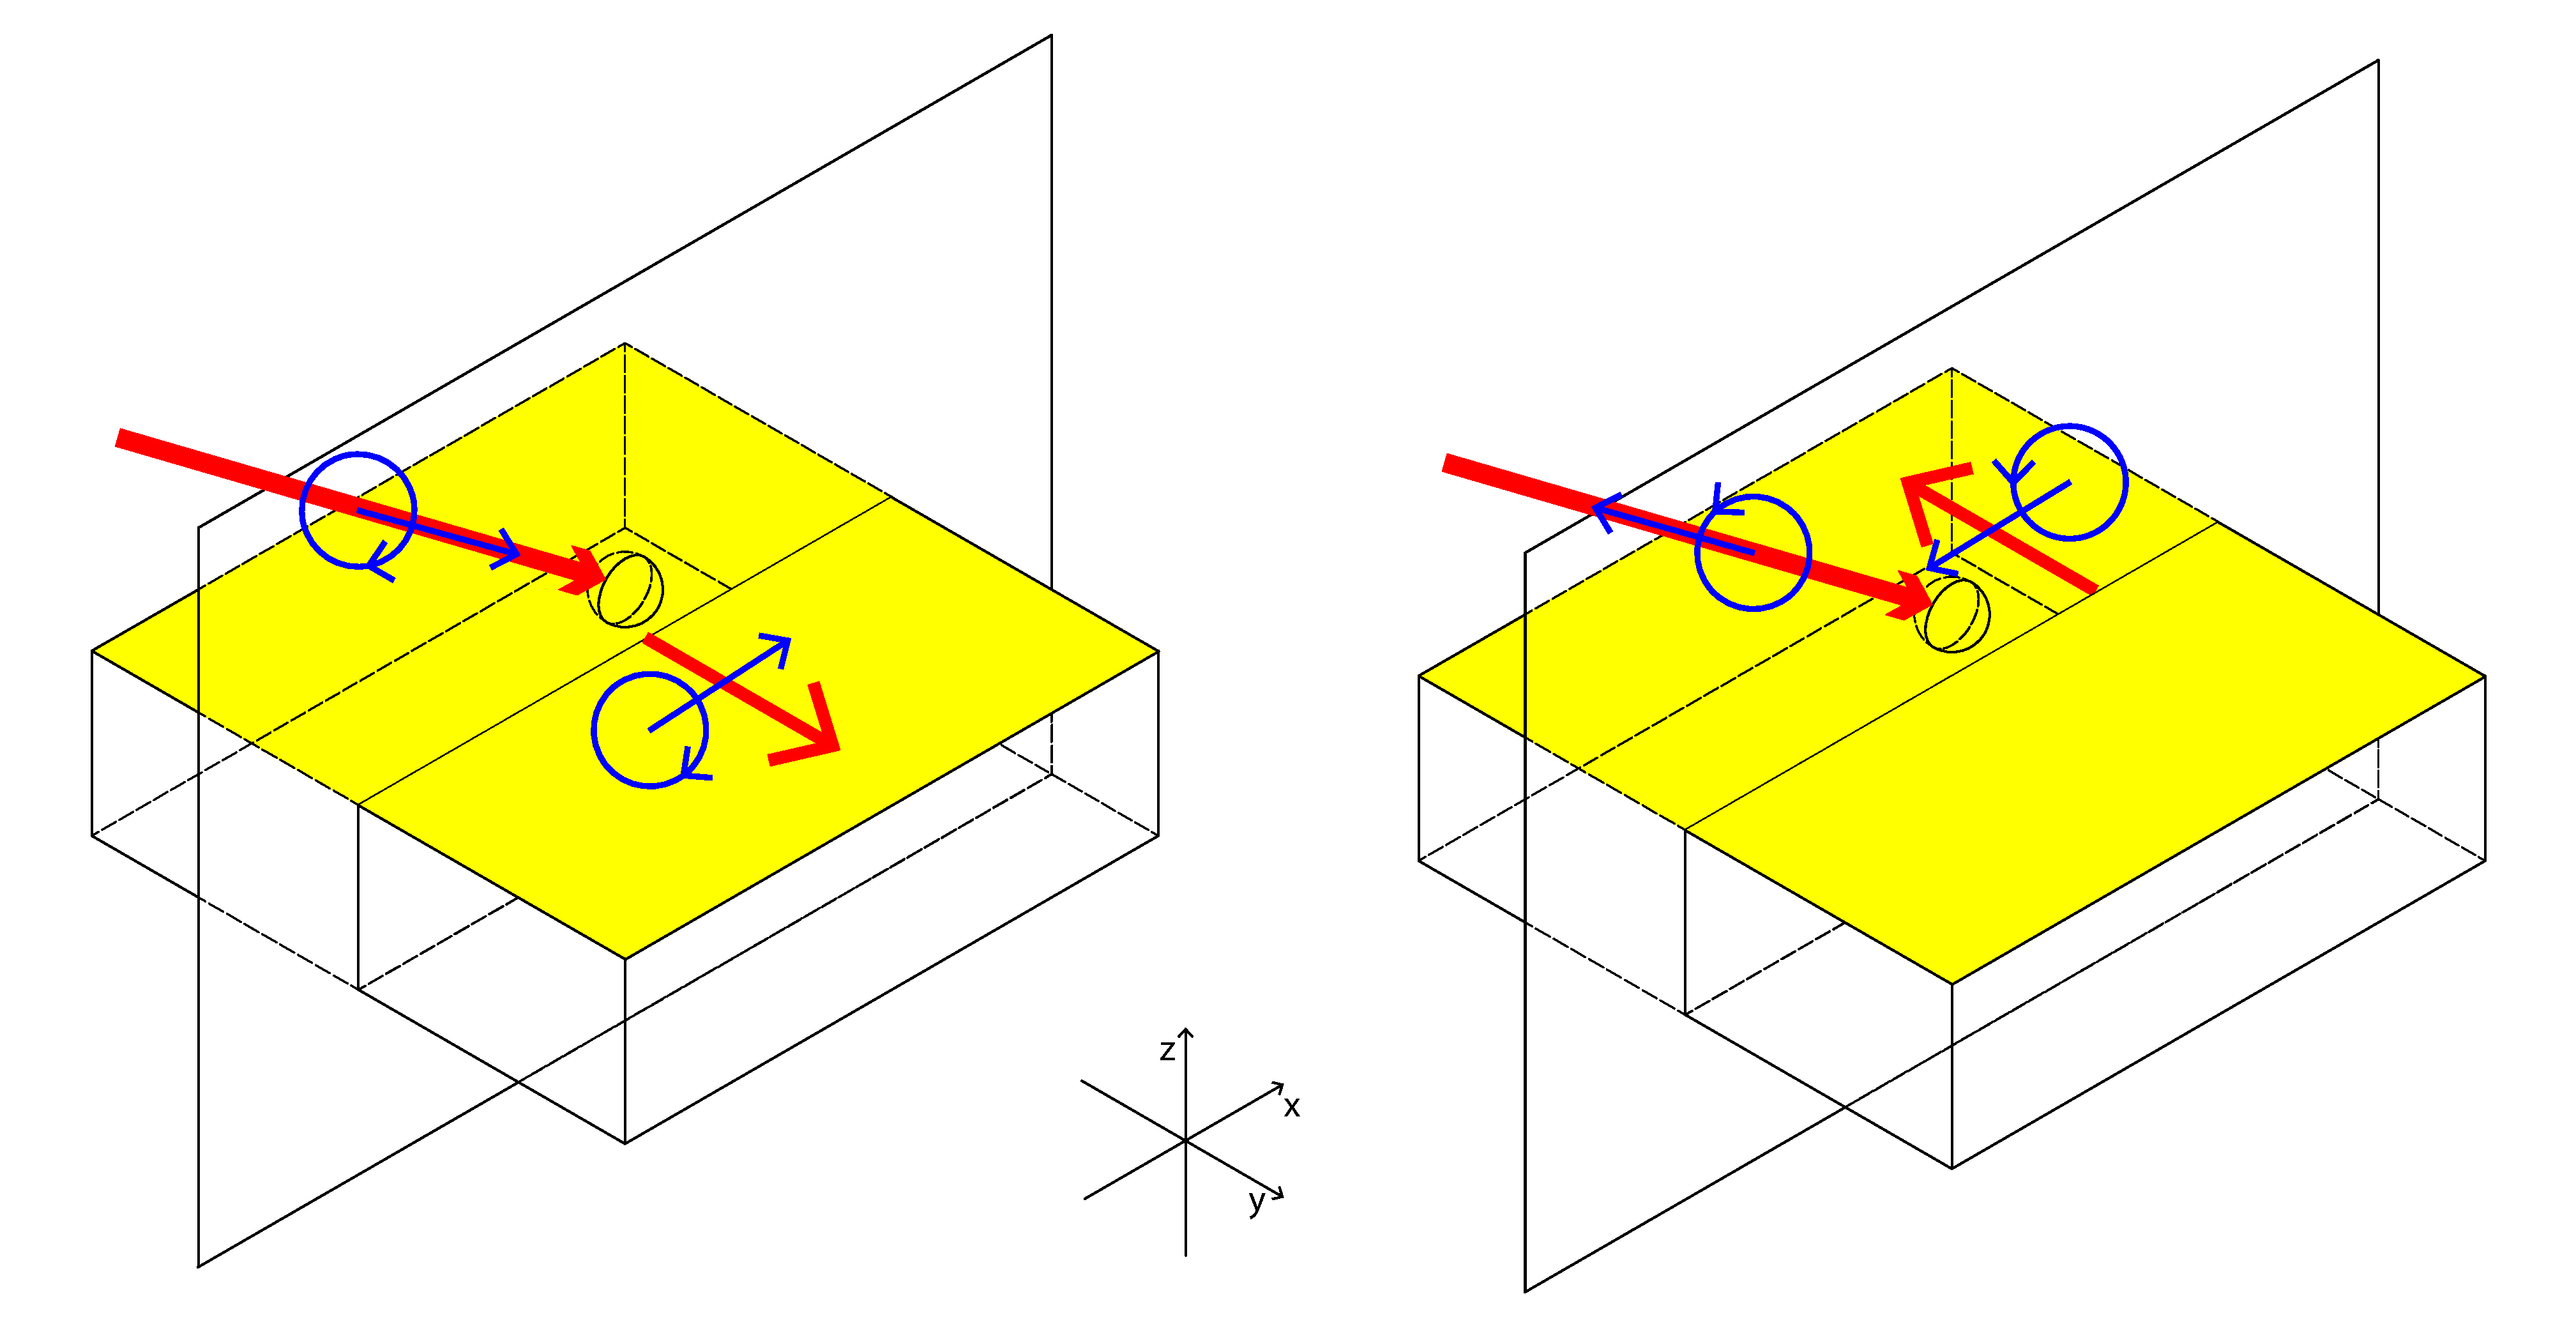
\includegraphics[width=1.0\linewidth]{figures/spin_hall_schema.pdf}
		\end{frame}
	
		\begin{frame}
			\frametitle{Raumfrequenzdarstellung Elektromagnetischer Strahlung}
			\begin{equation}
				\vec{E}(x,z) = 	\int_{-\infty}^{\infty}\mathrm{d}{k_x}\hat{\vec{E}}(k_x,z)\exp(ik_xx)			
			\end{equation}
			\begin{equation}
				\hat{\vec{E}}(k_x,z) = 	\dfrac{1}{2\pi}\int_{-\infty}^{\infty}\mathrm{d}x\vec{E}(x,z)\exp(-ik_xx)
			\end{equation}
				Medium entlang der $x$-Achse homogen, isotrop, linear und quellfrei:
		 	\begin{equation}
			 	\hat{\vec{E}}(k_x,z) =\hat{\vec{E}}(k_x,z= 0) \exp(\pm ik_ z)
			 \end{equation}
		 		mit:
		 	\begin{equation}
		 		k_z := \sqrt{k^2-k_x^2}
		 	\end{equation}		
		\end{frame}
	
		\begin{frame}
			\frametitle{Raumfrequenzspektrum zirkular polarisierter Dipol}
			\begin{center}
				\includegraphics[width=0.7\textwidth]{figures/spatial_spectrum_circ.pdf}	
			\end{center}				
		\end{frame}
	\section{Experimenteller Aufbau}
	\begin{frame}
		\frametitle{Aufbau}
		\begin{center}
				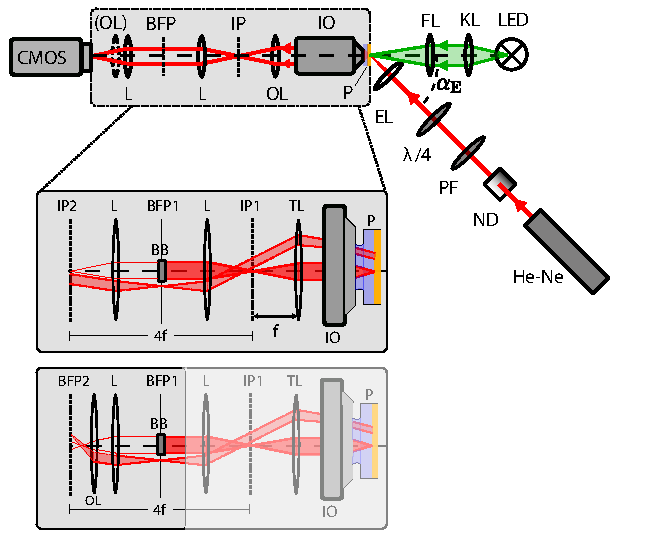
\includegraphics[width=0.7\textwidth]{figures/Aufbau_Schema.pdf}	
		\end{center}
	\end{frame}
	
	\begin{frame}
		\frametitle{Experimenteller Aufbau}
	\begin{center}
		\includegraphics[width=\textwidth]{figures/aufsicht_aufbau_anotated.jpg}
	\end{center}
		
	\end{frame}
	\begin{frame}
	\frametitle{Kontrolle der Polarisation des Anregungslasers}
		\begin{columns}
			\begin{column}{0.5\textwidth}
				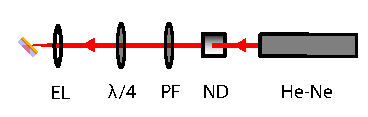
\includegraphics[width=\textwidth]{figures/polarisation_sheme.pdf}
			\end{column}
			\begin{column}{0.5\textwidth}  %%<--- here
				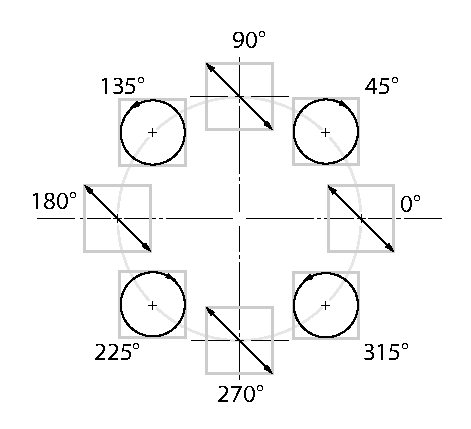
\includegraphics[width=\textwidth]{figures/Polarisation_lambda.pdf}
			\end{column}
		\end{columns}	
	\end{frame}
	\section{Messung und Ergebnisse}
		\subsection{Kontrollmessung}
			\begin{frame}
				\frametitle{Kontrollmessung an Punktdefekt}
				\begin{columns}
					\begin{column}{0.5\textwidth}
							\includegraphics[width=\textwidth]{figures/example_polar.png}
					\end{column}
					\begin{column}{0.5\textwidth}  %%<--- here
						\includegraphics[width=\textwidth]{figures/example_focal_plane.png}
					\end{column}
				\end{columns}
			\end{frame}
			
			\begin{frame}
				\frametitle{Auswertung der BFP}
				\begin{columns}
					\begin{column}{0.5\textwidth}
						\includegraphics[width=\textwidth]{figures/example_radial.pdf}
					\end{column}
					\begin{column}{0.5\textwidth}  %%<--- here
						\includegraphics[width=\textwidth]{figures/lorenz_profile.pdf}
					\end{column}
				\end{columns}
			\end{frame}
		\subsection{Experimenteller Nachweis des PSHE}
			\begin{frame}
				\frametitle{Rückwärtsrichtung}
				\begin{columns}
					\begin{column}{0.5\textwidth}
						\includegraphics[width=\textwidth]{figures/spin_hall/diff_back.png}
					\end{column}
					\begin{column}{0.5\textwidth}  %%<--- here
						\includegraphics[width=\textwidth]{figures/spin_hall/intensity_back.pdf}
					\end{column}
				\end{columns}
			\end{frame}
			\begin{frame}
				\frametitle{Vorwärtsrichtung}
				\begin{columns}
					\begin{column}{0.5\textwidth}
						\includegraphics[width=\textwidth]{figures/spin_hall/diff_forw.png}
					\end{column}
					\begin{column}{0.5\textwidth}  %%<--- here
						\includegraphics[width=\textwidth]{figures/spin_hall/intensity_forw.pdf}
					\end{column}
				\end{columns}
			\end{frame}
			\begin{frame}
				\frametitle{Senkrecht zur Einfallsebene}
				\begin{columns}
					\begin{column}{0.5\textwidth}
						\includegraphics[width=\textwidth]{figures/spin_hall/diff_mid.png}
					\end{column}
					\begin{column}{0.5\textwidth}  %%<--- here
						\includegraphics[width=\textwidth]{figures/spin_hall/intensity_mid.pdf}
					\end{column}
				\end{columns}
			\end{frame}
		
	
		
	
	

	
\end{document}